\documentclass[CJKutf8,dvipsnames,table]{beamer}
\usepackage{hyperref}
\hypersetup{
  pdfpagemode={FullScreen},
  colorlinks={true},
  linkcolor={blue},
}

%% https://tex.stackexchange.com/questions/47576/combining-ifxetex-and-ifluatex-with-the-logical-or-operation
\usepackage{iftex}
\newif\ifxetexorluatex % a new conditional starts as false
\ifnum 0\ifxetex 1\fi\ifluatex 1\fi>0
   \xetexorluatextrue
\fi
\usepackage{ifplatform}
\ifxetexorluatex
	\usepackage[slantfont,boldfont]{xeCJK}
	\ifwindows
		\setCJKmainfont{SimSun} % Windows默认中文字体:中易宋体
	\else
		\ifmacosx
			\setCJKmainfont{STSong} % MacOS默认中文字体:华文宋体
		\else
			\setCJKmainfont{Noto Serif CJK SC} % Linux默认中文字体:思源宋体(By Adobe & Google)
		\fi
	\fi
\else
	\usepackage{CJKutf8}
\fi

\usetheme{Madrid}%{Warsaw}
\usecolortheme{default}

\setbeamertemplate{footline}[page number]{} %gets rid of bottom navigation bars
\setbeamertemplate{navigation symbols}{} %gets rid of navigation symbols

\title{数字信号处理}
\subtitle{第1章:介绍}
\author{洪明坚 \hspace{1mm} 桑军}
\institute{重庆大学软件学院}
\date{\today}

\begin{document}
\ifxetexorluatex\else
\begin{CJK*}{UTF8}{song}
\fi

  \AtBeginSection[]
  {
    \begin{frame}
      \frametitle{Outline}
      \tableofcontents[currentsection]
    \end{frame}
  }

  \frame{\titlepage}
  \frame{\frametitle{目录}\tableofcontents}
  
  \section{课程介绍}
  
  %% PAGE
  \begin{frame}
    \frametitle{课程信息}
    \begin{itemize}
    \item 课程类别:专业基础课,3学分
    \item 教学形式:
      \begin{itemize}
      \item 课堂40学时 
      \item 实验16学时,Matlab 
      \end{itemize}
    \item 前导课程:
      \begin{itemize}
      \item 高等数学 
      \item 线性代数 
      \item {\color{red} 复变函数}
      \item Matlab
      \end{itemize}      
    \end{itemize}
  \end{frame}
  
  %% PAGE
  \begin{frame}
    \frametitle{课程内容} 
    \begin{itemize}
    \item 考虑到实际的开课情况,不求大而全,以有所收获为目的
        \begin{itemize}
        \item 信号 
        \item 系统  
        \item 傅立叶变换 
        \item 频域分析 
        \item 采样 
        \item 应用
        \end{itemize}
    \end{itemize}
  \end{frame}

  %% PAGE
  \begin{frame}
    \frametitle{参考书}
    \begin{itemize}
    \item 信号与系统(第2版),Alan V. Oppenheim等著,刘树棠 译
    \item 数字信号处理——基于计算机的方法(第4版),Sanjit K. Mitra著,余翔宇 译
    \end{itemize}
    \begin{center}
      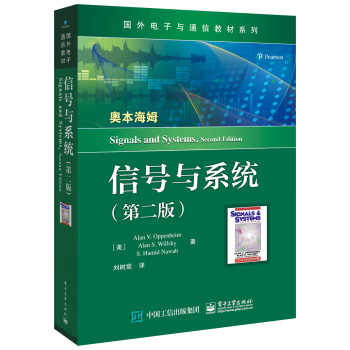
\includegraphics[scale=.31]{signalsandsystems}
      \hspace{1mm}
      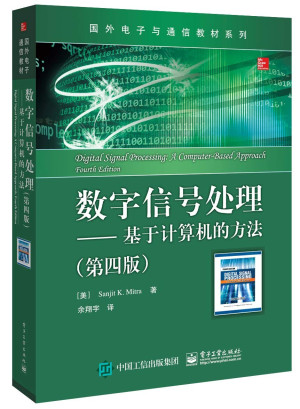
\includegraphics[scale=.35]{mitradsp}
    \end{center}
  \end{frame}
  
  %% PAGE
  \begin{frame}
    \frametitle{成绩}
    \begin{itemize}
    \item 总成绩 = 考勤 + 实验 + 期末考试
        \begin{itemize}   
        \item 各项具体占比待定
        \item 实验通过sakai提交报告 
        \end{itemize}
    \end{itemize}
  \end{frame}

  %% PAGE
  \begin{frame}
    \frametitle{Questions}
    \begin{itemize}
    \item Any questions?
    \end{itemize}
    \begin{center}
      
\includegraphics[scale=.5]{question}
    \end{center}
  \end{frame}
  
  \section{数学准备}
  
  %% PAGE
  \begin{frame}
    \frametitle{复数} 
    \begin{itemize}
    \item 虚数单位:${\color{red}j}=i=\sqrt{-1}$
    \item 任意复数:$z=x+jy=re^{j\theta}$
        \begin{itemize}
        \item $x=Re\{z\}, y=Im\{z\}$
        \item $x=r cos\theta, y=r sin\theta$
        \item $r=|z|=\sqrt{x^2+y^2}$是$z$的幅值(Magnitude),$\theta=Arg\{z\}$是z的相位(Phase)
        \item $\bar{z}=x-jy$是$z$的共轭(Conjugate)复数,$|\bar{z}|=|z|$。
        \end{itemize}
    \item 欧拉(Euler)公式
        \begin{itemize}
        \item $e^{j\theta}=cos\theta+jsin\theta$
        \item $e^{j\theta}$以$2\pi$为周期,且幅值$|e^{j\theta}|=1$
        \end{itemize}
    \item 棣莫弗(de Moivre)公式
        \begin{itemize}
        \item ${(e^{j\theta})}^n={(cos\theta+jsin\theta)}^n=cos(n\theta)+jsin(n\theta)$
        \end{itemize}    
    \end{itemize}
  \end{frame}  
  
  %% PAGE
  \begin{frame}
    \frametitle{常用公式} 
    \begin{itemize}
    \item 有限项和公式:
    	\[
\sum_{n=0}^{N-1}\alpha^n = 
\left\{
    \begin {aligned}
         & N \quad & \alpha=1 \\
         & \frac{1-\alpha^N}{1-\alpha} \quad & otherwise                  
    \end{aligned}
\right.
		\]        

    \item 无限项和公式:若$|\alpha|<1$,\[ \sum_{n=0}^{\infty}\alpha^n=\frac{1}{1-\alpha} \]   
    \end{itemize}
  \end{frame}  

\ifxetexorluatex\else
\end{CJK*}
\fi
\end{document}

%%% Local Variables: 
%%% mode: latex
%%% TeX-master: t
%%% End: 
